\documentclass[12pt]{article}

\usepackage[spanish,es-tabla]{babel}
\usepackage[utf8x]{inputenc}
\usepackage{amsmath}

\usepackage{hyperref}
\usepackage{url}
\usepackage{gensymb}
\usepackage[dvipsnames]{xcolor}

\usepackage{parskip}
\usepackage{fancyhdr}
\usepackage{multicol}
\usepackage{vmargin}
\usepackage{setspace}
\usepackage{geometry}

\usepackage{float}
\usepackage{array}
\usepackage{graphicx}
\graphicspath{{images/}}
\usepackage{wrapfig}
\usepackage{caption}
\usepackage{subcaption}

\setmarginsrb{2 cm}{1 cm}{2 cm}{1.5 cm}{1 cm}{1 cm}{1 cm}{1 cm}

\title{Determinación del coeficiente de compresibilidad isotérmica del aire}
\author{Martín Alejandro Paredes Sosa}		

\makeatletter
\let\thetitle\@title
\let\theauthor\@author
\let\thedate\@date										
\makeatother

\pagestyle{fancy}
\fancyhf{}
\rhead{Lic.. Física}
\lhead{Informe 4A}
\cfoot{\thepage}

\begin{document}
%%%%%%%%%%%%%%%%%%%%%%%%%%%%%%%%%%%%%%%%%%%%%%%%%%%%%%%%%%%%%%%%%%%%%%%%%%%%%%%%%%%%%%%%
%\begin{titlepage}
%	\centering
%    \vspace*{0.5 cm}
%    
\includegraphics[scale = 0.5]{logo}\\[0.5 cm]	% University Logo
%    \textsc{\LARGE Universidad de Sonora}\\[1 cm]	% University Name
%	\textsc{\Large División de Ciencias Exactas y Naturales}\\[1 cm]		%		% Course Code
%	\textsc{\large Termodinámica Clásica}\\[0.5 cm]				% Course Name
%	\rule{\linewidth}{0.2 mm} \\[0.4 cm]
\begin{center}
{ \large \bfseries \thetitle}\\
\end{center}
%{ \large \bfseries \thetitle}\\
%	\rule{\linewidth}{0.2 mm} \\[1.25 cm]
%    \textsc{\Large Equipo \#2} \\[1.25 cm]
%\thetitle\\	
	\begin{minipage}{\textwidth}
		\begin{center} 
			%\textsc{\Large Integrantes:} \large \\
			\theauthor 
			\end{center}
	\end{minipage}\\[-0.52 cm]
%===================================================================================================
\begin{abstract}
	Esta experiencia se utilizó el ``Aparato de ley adiabatica", con el cual se midió presión, volumen y temperatura. La idea es mantener una temperatura constante en el aparato, para así poder realizar las mediciones con las que se espera obtener el coeficiente de compresibilidad isotérmica del aire.

\end{abstract}
\vspace{-1cm}
%===================================================================================================
\section{Introducción}
	Para nuestra cuarta experiencia en el laboratorio, se nos presentó el ``Aparato de ley adiabatica'', con el objetivo de determinar el coeficiente de determinar el coeficiente de compresibilidad isotérmica del aire ($\kappa$).
	
\hspace{0.75cm}	Este dispositivo consiste en un cilindro de acrílico y un pistón, con válvulas para encerrar el gas que se desea estudiar. Este cuenta con 3 sensores, con los cuales utilizando DataStudio se midió el volumen, presión y temperatura.

\hspace{0.75cm} Un proceso adiabático es aquel en que el sistema no pierde ni gana calor. Es decir, que en la primera ley de la termodinámica, Q=0. El sistema si puede cambiar su estado si se realiza trabajo termodinámico.

%===================================================================================================
\section{Desarrollo Experimental}
Primeramente se instalo el aparato, es decir se conecto el dispositivo y se configuro el software para los sensores que se utilizarían.
\begin{figure}[H]\label{config}
\centering
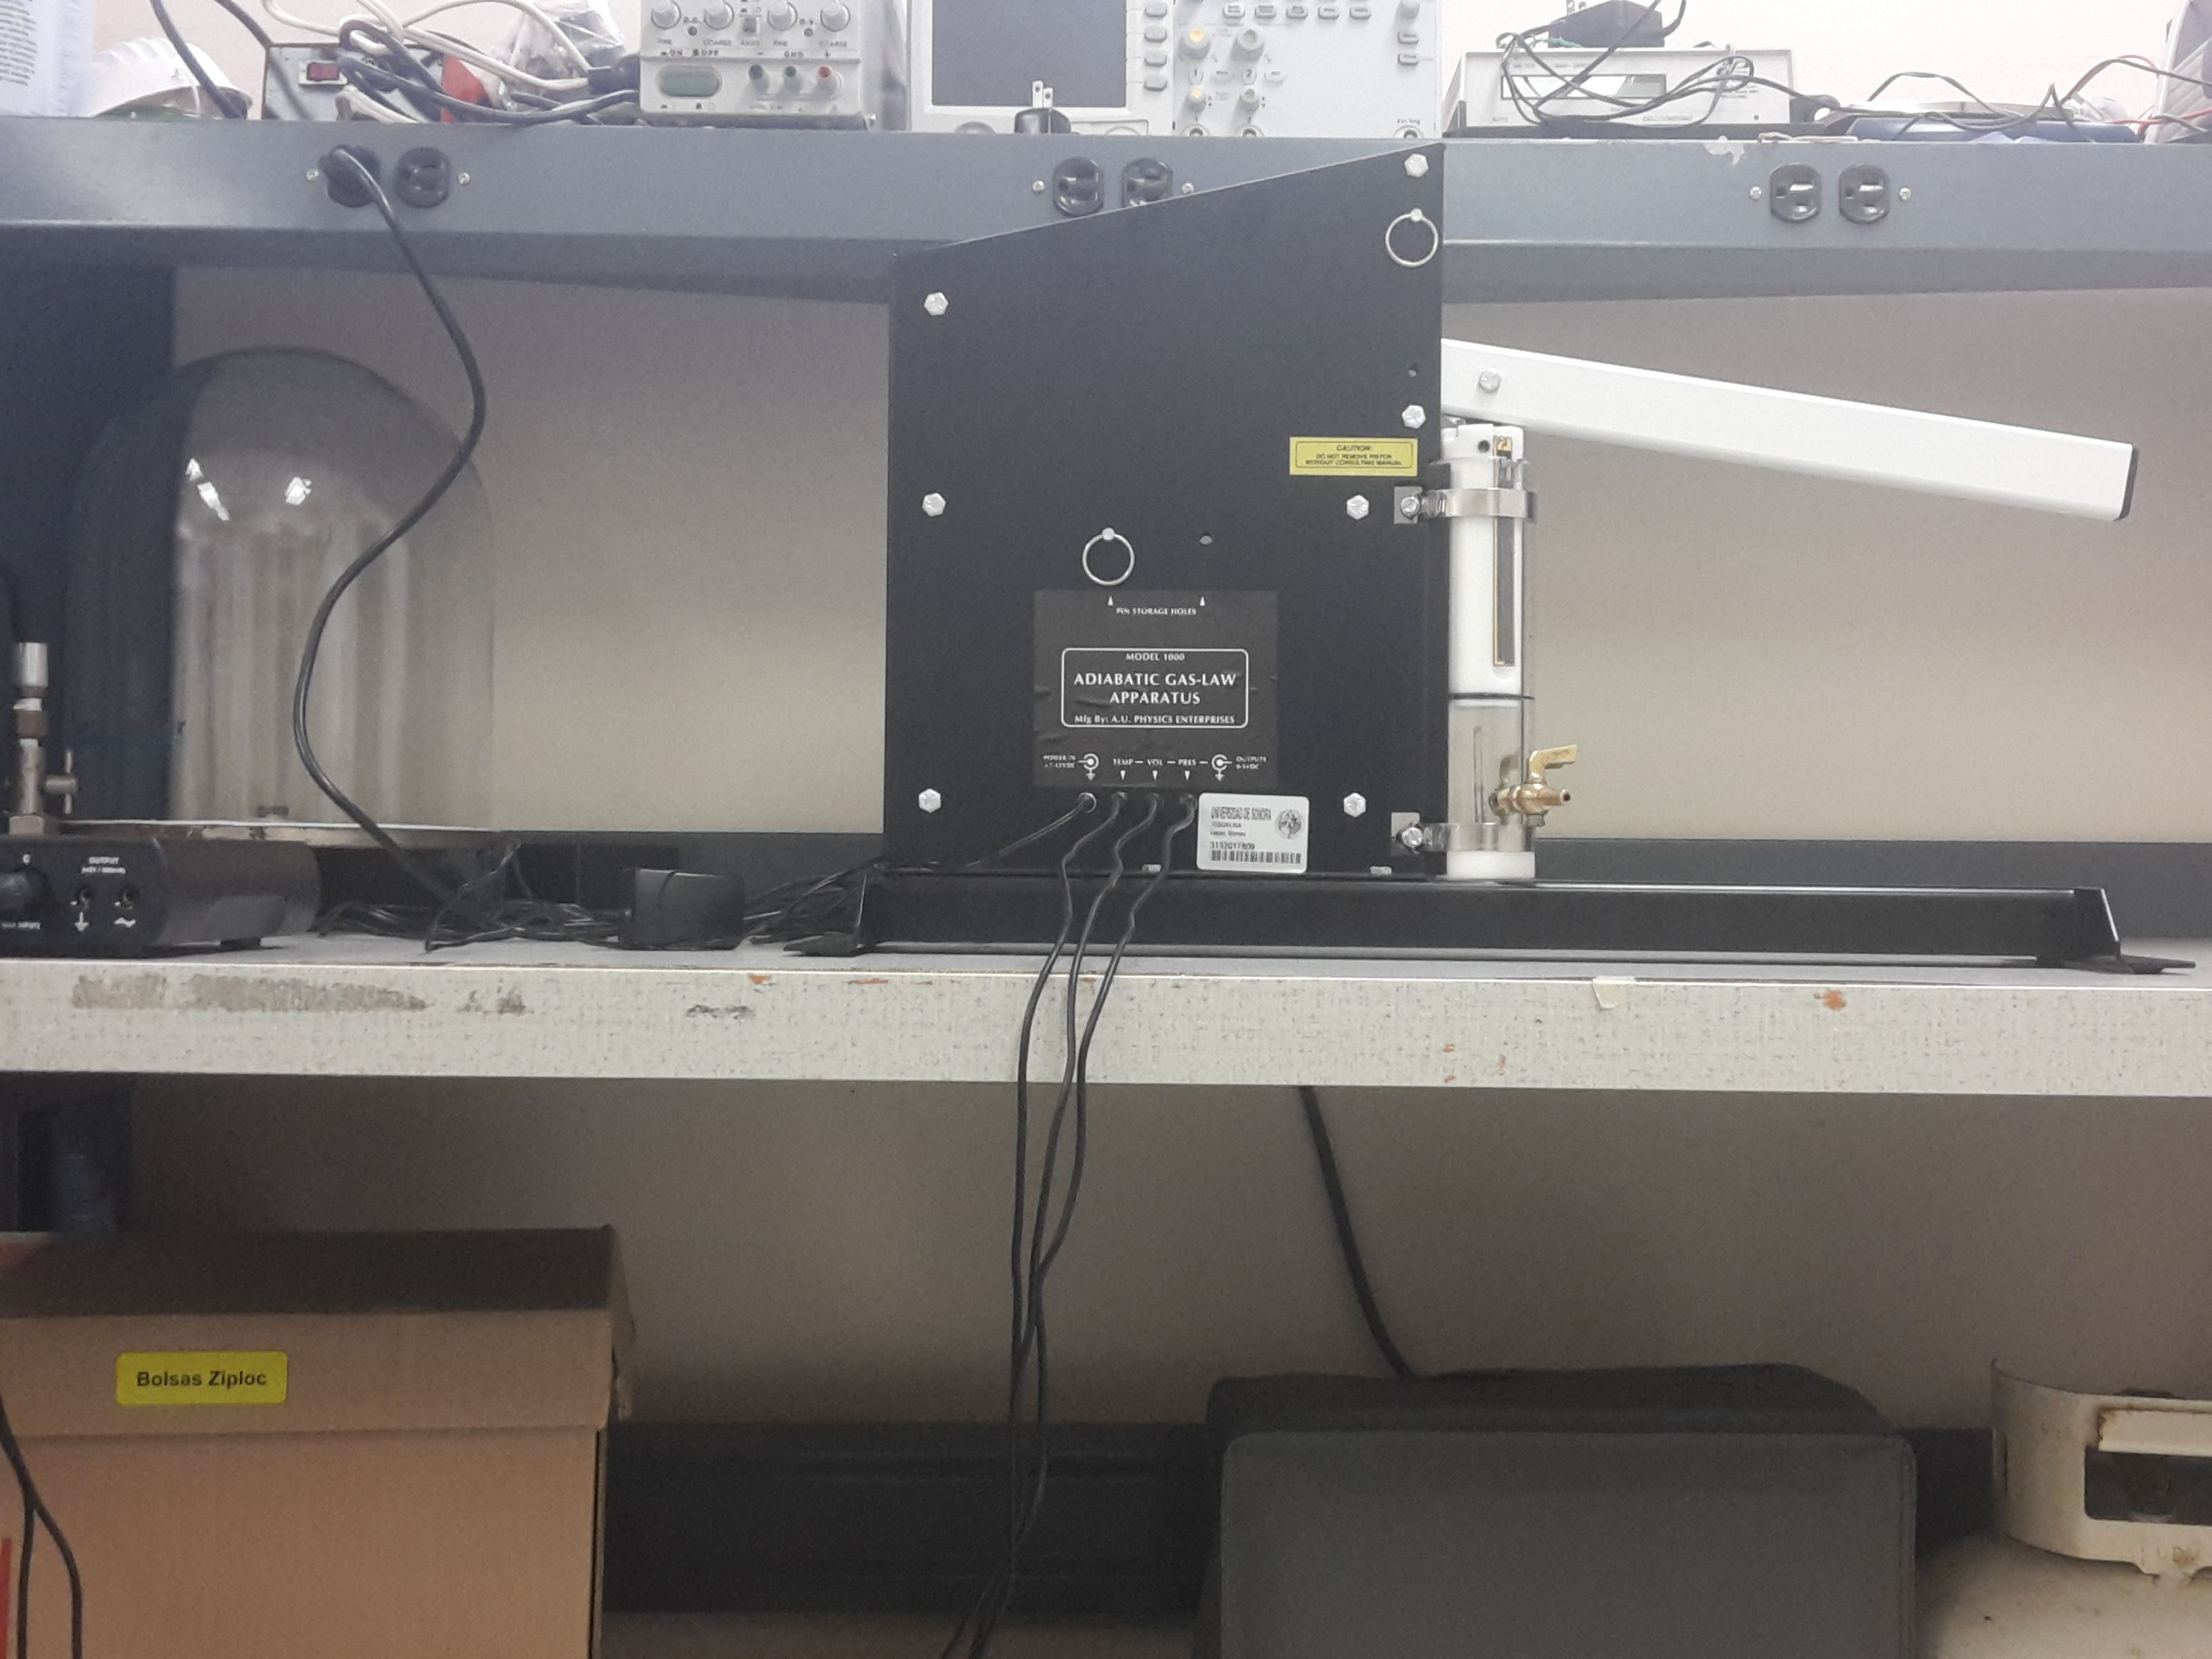
\includegraphics[width=0.45\linewidth]{config.jpg}
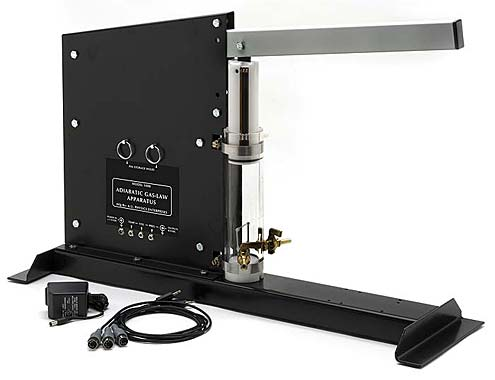
\includegraphics[width=0.45\linewidth]{aparato.jpg}
\caption{Arreglo Experimental}
\end{figure}
\pagebreak
Para calibrar este aparato se utilizan las siguientes expresiones:
\begin{itemize}
	\item \textbf{Presión Absoluta}$$P(V_P) = 100 V_m (kPa)$$
	\item \textbf{Volumen} $$ P(V_V) = 3.22\times 10^{-5}V_m + 8.28\times 10^{-5} (m^3) $$
	\item \textbf{Temperatura Absoluta} $$ T(V_T) = 68.86V_T +238.0 (K) $$
\end{itemize}
donde $V_V$, $V_P$ y $V_T$ son los voltajes obtenidos de los sensores.

\hspace{0.75cm}Se establecieron en dos referencias para la presión y el volumen (el mínimo y máximo alcance del movimiento del pistón). Se tomó lectura de los datos para obtener la referencia.

\hspace{0.75cm} Luego de obtener una referencia, se empezó a realizar una descompresión del volumen. Durante la descompresión se inicio una toma de datos de temperatura, volumen y presión con una frecuencia de muestro de 10Hz. Se trato de mantener la temperatura constante realizando la descompresión de manera lenta.

Como el objetivo es obtener el coeficiente kappa, el cual esta dado por:
\begin{equation}\label{kappa}
\kappa = \frac{-1}{V} \left( \frac{\partial V}{\partial P} \right) _{\theta}
\end{equation}
\hspace{0.75cm} Esto significa que se debe variar el volumen respecto a la presión maniendo una temperatura constante. Para lograr un proceso isotermo se procedió realizar movimientos lentos de la palanca del pistón; esto mantiene el valor de la temperatura cerca del valor promedió. Se realizaron 3 mediciones de la presión y el volumen manteniendo la temperatura constante.

Para obtener $\kappa$ es necesario realizar modificaciones a \eqref{kappa}.
\begin{equation}
\kappa = \frac{-1}{V} \left( \frac{\partial V}{\partial P} \right) _{\theta}
\end{equation}

\begin{equation}
\kappa = -\left( \frac{\partial \ln(V)}{\partial P} \right) _{\theta}
\end{equation}
Para poder aplicar el logaritmo, se tiene que volver adimensional su argumento dividiendo entre  el volumen inicial $V_0$ quedando:
\begin{equation}
\kappa = -\left( \frac{\partial \ln \left(\frac{V}{V_0} \right)  }{\partial P} \right) _{\theta}
\end{equation}
\pagebreak
%===================================================================================================
\section{Resultados}
Los valores de referencia que se obtuvieron se presentan en la siguiente tabla:

\begin{table}[H]
\centering
\begin{tabular}{|c|c|c|}
\hline
Medición  & Referencia 1  & Referencia 2 \\ \hline
   Presión     & 117.19$\pm15.51$ kPa& 209.63$\pm 5.09$ kPa \\ \hline
   Volumen &1.967$\pm0.014\times 10^{-4}$ $m^3$ &  9.502$\pm0.014\times 10^{-5}$ $m^3$  \\ \hline
   Temperatura  &  298.84 $\pm0.03$  K  &       \\ \hline
      
\end{tabular}
\caption{Medición de Referencias}
\end{table}
El comportamiento de la temperatura durante la medición de temperatura se muestra en la figura(2).
\begin{figure}[H]
\centering
%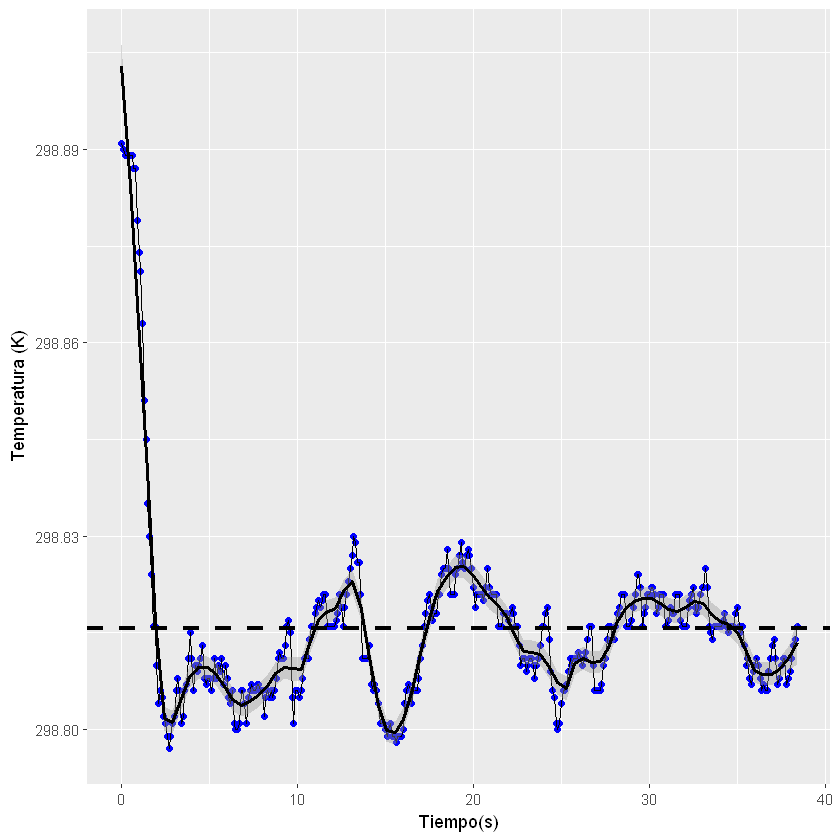
\includegraphics[width= 0.75\linewidth]{temperatura.png}
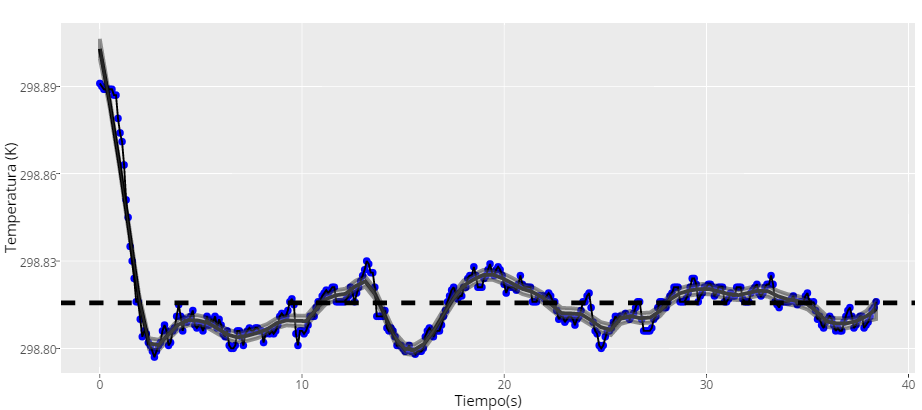
\includegraphics[width= 0.75\linewidth]{newplot.png}
\caption{Comportamiento de la Temperatura}
\end{figure}
\hspace{0.75cm}
Se puede observar que los datos al principio tuvieron una variación de tamaños considerable.

 Para obtener $\kappa$ se debe ver el comportamiento del $ \ln \left(\frac{V}{V_0} \right)$ con respecto a la presión como se muestra en la siguiente figura.

\begin{figure}[H]
	\centering
	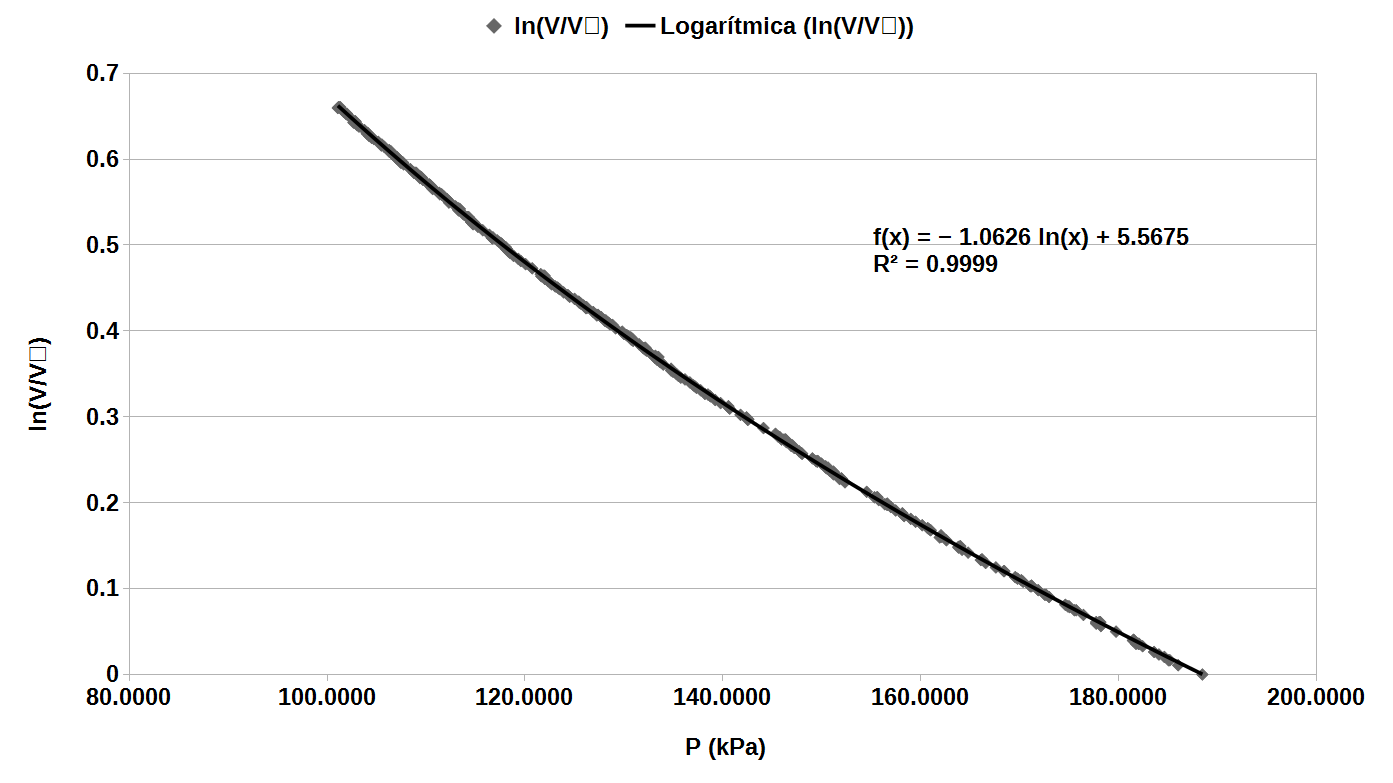
\includegraphics[width=0.75\linewidth]{kappaObt}
	\caption{Relación $ \ln \left(\frac{V}{V_0} \right)$ vs P}
\end{figure}
Como se puede observar del gráfico, el proceso fue una expansión ya que el logaritmo natural se hace 0 en la mayor presión. A partir de la forma de los datos, se realizo un ajuste logarítmico.
\begin{equation}
\left(\ln \left(\frac{V}{V_0} \right) \right)_{\theta} = -1.0626\cdot\ln(kPa) + 5.5675; \hspace{1.5cm} R^2 = 0.9999
\end{equation}
Es decir, kappa seria:
$$\kappa = 1.0626 \cdot \ln(kPa) $$

%En el apéndice se pueden encontrar los datos experimentales y mas graficas del comportamiento observado.
\pagebreak


%===================================================================================================
\section{Discusión}
Si modelamos al aire como gas ideal, su ecuación de estado es $PV=nR\theta$.
$$\kappa = -\frac{1}{V} \left( \frac{\partial V}{\partial P} \right) _{\theta} = -\frac{1}{V} \left( \frac{\partial \frac{nR\theta}{P})}{\partial P} \right) _{\theta} = \frac{1}{P}$$
Por lo que kappa en el gas ideal tiene comportamiento de hipérbola, mientras que el que se obtuvo es una función logaritmo natural. Se puede decir que en las condiciones en la que se encontraba el aire, no es un gas ideal.
%===================================================================================================
\section{Conclusiones}
Se puede concluir que para mejores resultados, se ocupa realizar el experimento en intervalos grandes de tiempo, así se pude lograr una mejor obtención de una temperatura constante y se tienen mas datos para realizar el análisis.

%================================================================================================
\begin{thebibliography}{6}
\bibitem{a}
	Rodríguez Mellado, J.M. (s.f.) \textit{Coeficientes de dilatación térmica y de compresibilidad isotérmico} Recuperado el 19 de Febrero 2017 de	\url{http://www.uco.es/~qf1romej/termodinamica/docs/alfaykappa.pdf}
	
\bibitem{acu}
Acu\~na, H. (2015). \textit{Manual de Guías de Experiencias en el Laboratorio de Termodinámica Clásica}.

\end{thebibliography}
\pagebreak
%================================================================================================
\section{Apendice}
\vspace{-0.5cm}
\begin{table}[H]
\centering
\begin{tabular}{|c|c|c|c|}
\hline
Tiempo ( s ) & T ( K )  & V ( m3 )   & P ( kPa ) \\ \hline
0.0000       & 298.8910 & 9.5050E-05 & 204.5350  \\ \hline
0.1000       & 298.8900 & 9.5080E-05 & 204.4740  \\ \hline
0.2000       & 298.8890 & 9.5060E-05 & 204.5350  \\ \hline
0.3000       & 298.8890 & 9.5080E-05 & 204.4740  \\ \hline
0.4000       & 298.8890 & 9.5080E-05 & 204.4130  \\ \hline
0.5000       & 298.8890 & 9.5080E-05 & 204.4130  \\ \hline
0.6000       & 298.8890 & 9.5080E-05 & 204.3520  \\ \hline
0.7000       & 298.8870 & 9.5080E-05 & 204.2300  \\ \hline
0.8000       & 298.8870 & 9.5160E-05 & 204.0470  \\ \hline
0.9000       & 298.8790 & 9.5740E-05 & 202.3380  \\ \hline
1.0000       & 298.8740 & 9.5800E-05 & 202.2160  \\ \hline
1.1000       & 298.8710 & 9.6170E-05 & 201.1780  \\ \hline
1.2000       & 298.8630 & 9.6970E-05 & 199.2250  \\ \hline
1.3000       & 298.8510 & 9.7920E-05 & 196.8440  \\ \hline
1.4000       & 298.8450 & 9.8410E-05 & 195.7460  \\ \hline
1.5000       & 298.8350 & 9.9440E-05 & 192.9380  \\ \hline
1.6000       & 298.8300 & 9.9560E-05 & 192.8160  \\ \hline
1.7000       & 298.8240 & 1.0070E-04 & 190.3740  \\ \hline
1.8000       & 298.8160 & 1.0150E-04 & 188.6650  \\ \hline
1.9000       & 298.8160 & 1.0170E-04 & 188.4820  \\ \hline
2.0000       & 298.8100 & 1.0280E-04 & 186.0410  \\ \hline
2.1000       & 298.8040 & 1.0340E-04 & 185.0640  \\ \hline
2.2000       & 298.8060 & 1.0340E-04 & 185.1860  \\ \hline
2.3000       & 298.8050 & 1.0380E-04 & 184.6370  \\ \hline
2.4000       & 298.8020 & 1.0410E-04 & 184.0880  \\ \hline
2.5000       & 298.8010 & 1.0440E-04 & 183.5990  \\ \hline
2.6000       & 298.7990 & 1.0510E-04 & 182.4400  \\ \hline
2.7000       & 298.7970 & 1.0540E-04 & 181.7680  \\ \hline
2.8000       & 298.7990 & 1.0540E-04 & 182.0120  \\ \hline
2.9000       & 298.8010 & 1.0540E-04 & 182.0730  \\ \hline
3.0000       & 298.8020 & 1.0580E-04 & 181.5850  \\ \hline
3.1000       & 298.8060 & 1.0580E-04 & 181.4630  \\ \hline
3.2000       & 298.8080 & 1.0590E-04 & 181.5240  \\ \hline
3.3000       & 298.8060 & 1.0690E-04 & 179.7540  \\ \hline
3.4000       & 298.8010 & 1.0760E-04 & 178.2280  \\ \hline
3.5000       & 298.8020 & 1.0790E-04 & 177.7400  \\ \hline
3.6000       & 298.8060 & 1.0810E-04 & 177.7400  \\ \hline
3.7000       & 298.8070 & 1.0810E-04 & 177.8010  \\ \hline
3.8000       & 298.8110 & 1.0810E-04 & 178.0450  \\ \hline
3.9000       & 298.8150 & 1.0810E-04 & 178.1670  \\ \hline
4.0000       & 298.8110 & 1.0900E-04 & 176.4580  \\ \hline
4.1000       & 298.8060 & 1.0960E-04 & 175.5420  \\ \hline
4.2000       & 298.8100 & 1.0960E-04 & 175.7260  \\ \hline
4.3000       & 298.8090 & 1.1000E-04 & 175.0540  \\ \hline

\end{tabular}

\end{table}
\pagebreak
\begin{table}[H]
\centering
\begin{tabular}{|c|c|c|c|}
\hline
Tiempo ( s ) & T ( K )  & V ( m3 )   & P ( kPa ) \\ \hline
4.4000       & 298.8100 & 1.1010E-04 & 174.8710  \\ \hline
4.5000       & 298.8110 & 1.1010E-04 & 174.9930  \\ \hline 
4.6000       & 298.8130 & 1.1030E-04 & 174.6270  \\ \hline
4.7000       & 298.8080 & 1.1130E-04 & 172.9790  \\ \hline
4.8000       & 298.8070 & 1.1160E-04 & 172.5520  \\ \hline
4.9000       & 298.8080 & 1.1160E-04 & 172.6740  \\ \hline
5.0000       & 298.8080 & 1.1220E-04 & 171.8800  \\ \hline
5.1000       & 298.8060 & 1.1270E-04 & 171.0870  \\ \hline
5.2000       & 298.8080 & 1.1270E-04 & 171.2090  \\ \hline
5.3000       & 298.8110 & 1.1280E-04 & 171.2090  \\ \hline
5.4000       & 298.8080 & 1.1330E-04 & 170.3540  \\ \hline
5.5000       & 298.8100 & 1.1350E-04 & 170.1710  \\ \hline
5.6000       & 298.8090 & 1.1370E-04 & 169.8050  \\ \hline
5.7000       & 298.8110 & 1.1390E-04 & 169.5610  \\ \hline
5.8000       & 298.8070 & 1.1470E-04 & 168.4620  \\ \hline
5.9000       & 298.8100 & 1.1470E-04 & 168.4010  \\ \hline
6.0000       & 298.8080 & 1.1520E-04 & 167.6080  \\ \hline
6.1000       & 298.8050 & 1.1580E-04 & 166.5700  \\ \hline
6.2000       & 298.8040 & 1.1620E-04 & 166.0820  \\ \hline
6.3000       & 298.8060 & 1.1630E-04 & 166.2040  \\ \hline
6.4000       & 298.8010 & 1.1720E-04 & 164.8000  \\ \hline
6.5000       & 298.8000 & 1.1760E-04 & 164.1900  \\ \hline
6.6000       & 298.8000 & 1.1790E-04 & 163.8230  \\ \hline
6.7000       & 298.8010 & 1.1800E-04 & 163.8230  \\ \hline
6.8000       & 298.8060 & 1.1800E-04 & 163.9450  \\ \hline
6.9000       & 298.8060 & 1.1810E-04 & 164.0060  \\ \hline
7.0000       & 298.8040 & 1.1890E-04 & 162.6030  \\ \hline
7.1000       & 298.8010 & 1.1930E-04 & 161.9310  \\ \hline
7.2000       & 298.8050 & 1.1940E-04 & 162.1140  \\ \hline
7.3000       & 298.8060 & 1.1940E-04 & 162.1750  \\ \hline
7.4000       & 298.8070 & 1.1960E-04 & 162.0530  \\ \hline
7.5000       & 298.8060 & 1.2030E-04 & 161.0160  \\ \hline
7.6000       & 298.8060 & 1.2040E-04 & 160.8940  \\ \hline
7.7000       & 298.8070 & 1.2060E-04 & 160.7100  \\ \hline
7.8000       & 298.8070 & 1.2100E-04 & 160.1610  \\ \hline
7.9000       & 298.8060 & 1.2150E-04 & 159.4900  \\ \hline
8.0000       & 298.8060 & 1.2190E-04 & 159.0010  \\ \hline
8.1000       & 298.8020 & 1.2230E-04 & 158.3300  \\ \hline
8.2000       & 298.8050 & 1.2250E-04 & 158.2080  \\ \hline
8.3000       & 298.8060 & 1.2270E-04 & 158.1470  \\ \hline
8.4000       & 298.8050 & 1.2310E-04 & 157.4760  \\ \hline
8.5000       & 298.8060 & 1.2360E-04 & 156.9870  \\ \hline
8.6000       & 298.8050 & 1.2390E-04 & 156.6210  \\ \hline
8.7000       & 298.8060 & 1.2400E-04 & 156.3770  \\ \hline
\end{tabular}

\end{table}
\pagebreak
\begin{table}[H]
\centering
\begin{tabular}{|c|c|c|c|}
\hline
Tiempo ( s ) & T ( K )  & V ( m3 )   & P ( kPa ) \\ \hline
8.8000       & 298.8080 & 1.2400E-04 & 156.5600  \\ \hline
8.9000       & 298.8110 & 1.2410E-04 & 156.6210  \\ \hline
9.0000       & 298.8120 & 1.2410E-04 & 156.6210  \\ \hline
9.1000       & 298.8110 & 1.2460E-04 & 155.7660  \\ \hline
9.2000       & 298.8110 & 1.2500E-04 & 155.3390  \\ \hline
9.3000       & 298.8130 & 1.2500E-04 & 155.5830  \\ \hline
9.4000       & 298.8160 & 1.2500E-04 & 155.5830  \\ \hline
9.5000       & 298.8170 & 1.2500E-04 & 155.6440  \\ \hline
9.6000       & 298.8150 & 1.2580E-04 & 154.5460  \\ \hline
9.7000       & 298.8050 & 1.2720E-04 & 152.3480  \\ \hline
9.8000       & 298.8010 & 1.2770E-04 & 151.7990  \\ \hline
9.9000       & 298.8060 & 1.2770E-04 & 152.0430  \\ \hline
10.0000      & 298.8060 & 1.2780E-04 & 151.9820  \\ \hline
10.1000      & 298.8050 & 1.2840E-04 & 151.1890  \\ \hline
10.2000      & 298.8060 & 1.2850E-04 & 151.1890  \\ \hline
10.3000      & 298.8080 & 1.2850E-04 & 151.1890  \\ \hline
10.4000      & 298.8110 & 1.2850E-04 & 151.3110  \\ \hline
10.5000      & 298.8110 & 1.2880E-04 & 151.1890  \\ \hline
10.6000      & 298.8110 & 1.2890E-04 & 150.8220  \\ \hline
10.7000      & 298.8140 & 1.2900E-04 & 150.8220  \\ \hline
10.8000      & 298.8160 & 1.2920E-04 & 150.5780  \\ \hline
10.9000      & 298.8160 & 1.2940E-04 & 150.3950  \\ \hline
11.0000      & 298.8180 & 1.2940E-04 & 150.6390  \\ \hline
11.1000      & 298.8190 & 1.2960E-04 & 150.3950  \\ \hline
11.2000      & 298.8200 & 1.3000E-04 & 149.9680  \\ \hline
11.3000      & 298.8190 & 1.3030E-04 & 149.5410  \\ \hline
11.4000      & 298.8200 & 1.3040E-04 & 149.4190  \\ \hline
11.5000      & 298.8210 & 1.3040E-04 & 149.6020  \\ \hline
11.6000      & 298.8210 & 1.3080E-04 & 149.0520  \\ \hline
11.7000      & 298.8160 & 1.3150E-04 & 148.0150  \\ \hline
11.8000      & 298.8160 & 1.3160E-04 & 147.9540  \\ \hline
11.9000      & 298.8160 & 1.3190E-04 & 147.7100  \\ \hline
12.0000      & 298.8160 & 1.3240E-04 & 147.2210  \\ \hline
12.1000      & 298.8160 & 1.3270E-04 & 146.9160  \\ \hline
12.2000      & 298.8170 & 1.3280E-04 & 146.9160  \\ \hline
12.3000      & 298.8180 & 1.3280E-04 & 146.9770  \\ \hline
12.4000      & 298.8210 & 1.3280E-04 & 147.0380  \\ \hline
12.5000      & 298.8190 & 1.3330E-04 & 146.4280  \\ \hline
12.6000      & 298.8160 & 1.3370E-04 & 145.9400  \\ \hline
12.7000      & 298.8190 & 1.3370E-04 & 146.0010  \\ \hline
12.8000      & 298.8210 & 1.3370E-04 & 146.1840  \\ \hline
12.9000      & 298.8230 & 1.3370E-04 & 146.1840  \\ \hline
13.0000      & 298.8250 & 1.3370E-04 & 146.2450  \\ \hline
\end{tabular}

\end{table}
\pagebreak
\begin{table}[H]
\centering
\begin{tabular}{|c|c|c|c|}
\hline
Tiempo ( s ) & T ( K )  & V ( m3 )   & P ( kPa ) \\ \hline
13.1000      & 298.8270 & 1.3370E-04 & 146.3060  \\ \hline
13.2000      & 298.8300 & 1.3370E-04 & 146.3670  \\ \hline
13.3000      & 298.8290 & 1.3410E-04 & 145.7560  \\ \hline
13.4000      & 298.8260 & 1.3420E-04 & 145.5730  \\ \hline
13.5000      & 298.8260 & 1.3460E-04 & 145.3290  \\ \hline
13.6000      & 298.8210 & 1.3550E-04 & 144.1080  \\ \hline
13.7000      & 298.8110 & 1.3680E-04 & 142.5210  \\ \hline
13.8000      & 298.8110 & 1.3690E-04 & 142.5820  \\ \hline
13.9000      & 298.8110 & 1.3710E-04 & 142.3990  \\ \hline
14.0000      & 298.8110 & 1.3720E-04 & 142.3990  \\ \hline
14.1000      & 298.8130 & 1.3760E-04 & 141.7890  \\ \hline
14.2000      & 298.8070 & 1.3860E-04 & 140.6900  \\ \hline
14.3000      & 298.8060 & 1.3880E-04 & 140.5680  \\ \hline
14.4000      & 298.8070 & 1.3900E-04 & 140.5680  \\ \hline
14.5000      & 298.8060 & 1.3950E-04 & 139.7750  \\ \hline
14.6000      & 298.8040 & 1.4000E-04 & 139.2250  \\ \hline
14.7000      & 298.8010 & 1.4060E-04 & 138.7370  \\ \hline
14.8000      & 298.8010 & 1.4090E-04 & 138.4930  \\ \hline
14.9000      & 298.8010 & 1.4100E-04 & 138.1880  \\ \hline
15.0000      & 298.8000 & 1.4160E-04 & 137.7610  \\ \hline
15.1000      & 298.7990 & 1.4200E-04 & 137.3330  \\ \hline
15.2000      & 298.8000 & 1.4220E-04 & 137.2110  \\ \hline
15.3000      & 298.8010 & 1.4240E-04 & 137.0280  \\ \hline
15.4000      & 298.7990 & 1.4290E-04 & 136.6620  \\ \hline
15.5000      & 298.7990 & 1.4340E-04 & 136.1740  \\ \hline
15.6000      & 298.7980 & 1.4370E-04 & 135.7460  \\ \hline
15.7000      & 298.7990 & 1.4400E-04 & 135.5020  \\ \hline
15.8000      & 298.7990 & 1.4430E-04 & 135.3190  \\ \hline
15.9000      & 298.7990 & 1.4470E-04 & 134.9530  \\ \hline
16.0000      & 298.8000 & 1.4490E-04 & 134.7700  \\ \hline
16.1000      & 298.8040 & 1.4490E-04 & 134.8920  \\ \hline
16.2000      & 298.8060 & 1.4490E-04 & 134.9530  \\ \hline
16.3000      & 298.8070 & 1.4520E-04 & 134.7700  \\ \hline
16.4000      & 298.8060 & 1.4590E-04 & 133.9760  \\ \hline
16.5000      & 298.8040 & 1.4630E-04 & 133.7320  \\ \hline
16.6000      & 298.8060 & 1.4640E-04 & 133.6100  \\ \hline
16.7000      & 298.8060 & 1.4670E-04 & 133.3660  \\ \hline
16.8000      & 298.8060 & 1.4700E-04 & 133.1830  \\ \hline
16.9000      & 298.8080 & 1.4710E-04 & 133.1220  \\ \hline
17.0000      & 298.8110 & 1.4710E-04 & 133.2440  \\ \hline
17.1000      & 298.8130 & 1.4720E-04 & 133.2440  \\ \hline
17.2000      & 298.8160 & 1.4710E-04 & 133.3050  \\ \hline
17.3000      & 298.8180 & 1.4710E-04 & 133.3660  \\ \hline
17.4000      & 298.8200 & 1.4720E-04 & 133.4880  \\ \hline
17.5000      & 298.8210 & 1.4740E-04 & 133.1830  \\ \hline
\end{tabular}

\end{table}
\pagebreak
\begin{table}[H]
\centering
\begin{tabular}{|c|c|c|c|}
\hline
Tiempo ( s ) & T ( K )  & V ( m3 )   & P ( kPa ) \\ \hline
17.6000      & 298.8190 & 1.4800E-04 & 132.5720  \\ \hline
17.7000      & 298.8170 & 1.4830E-04 & 132.2670  \\ \hline
17.8000      & 298.8180 & 1.4850E-04 & 132.1450  \\ \hline
17.9000      & 298.8180 & 1.4870E-04 & 131.9620  \\ \hline
18.0000      & 298.8210 & 1.4870E-04 & 132.0230  \\ \hline
18.1000      & 298.8210 & 1.4870E-04 & 132.1450  \\ \hline
18.2000      & 298.8240 & 1.4870E-04 & 132.0840  \\ \hline
18.3000      & 298.8250 & 1.4870E-04 & 132.2060  \\ \hline
18.4000      & 298.8250 & 1.4870E-04 & 132.2670  \\ \hline
18.5000      & 298.8280 & 1.4880E-04 & 132.1450  \\ \hline
18.6000      & 298.8250 & 1.4940E-04 & 131.5350  \\ \hline
18.7000      & 298.8210 & 1.5000E-04 & 130.9240  \\ \hline
18.8000      & 298.8210 & 1.5020E-04 & 130.7410  \\ \hline
18.9000      & 298.8210 & 1.5020E-04 & 130.7410  \\ \hline
19.0000      & 298.8240 & 1.5030E-04 & 130.8630  \\ \hline
19.1000      & 298.8250 & 1.5030E-04 & 130.8630  \\ \hline
19.2000      & 298.8270 & 1.5030E-04 & 130.8630  \\ \hline
19.3000      & 298.8290 & 1.5040E-04 & 130.8020  \\ \hline
19.4000      & 298.8260 & 1.5060E-04 & 130.6800  \\ \hline
19.5000      & 298.8250 & 1.5090E-04 & 130.3750  \\ \hline
19.6000      & 298.8270 & 1.5100E-04 & 130.2530  \\ \hline
19.7000      & 298.8280 & 1.5110E-04 & 130.2530  \\ \hline
19.8000      & 298.8270 & 1.5120E-04 & 130.0090  \\ \hline
19.9000      & 298.8250 & 1.5160E-04 & 129.8260  \\ \hline
20.0000      & 298.8220 & 1.5220E-04 & 129.1540  \\ \hline
20.1000      & 298.8190 & 1.5280E-04 & 128.8490  \\ \hline
20.2000      & 298.8210 & 1.5290E-04 & 128.6050  \\ \hline
20.3000      & 298.8210 & 1.5310E-04 & 128.4830  \\ \hline
20.4000      & 298.8210 & 1.5320E-04 & 128.4220  \\ \hline
20.5000      & 298.8210 & 1.5340E-04 & 128.2390  \\ \hline
20.6000      & 298.8200 & 1.5360E-04 & 128.0560  \\ \hline
20.7000      & 298.8220 & 1.5350E-04 & 128.1170  \\ \hline
20.8000      & 298.8250 & 1.5360E-04 & 128.1780  \\ \hline
20.9000      & 298.8220 & 1.5420E-04 & 127.6890  \\ \hline
21.0000      & 298.8210 & 1.5450E-04 & 127.2620  \\ \hline
21.1000      & 298.8210 & 1.5460E-04 & 127.2620  \\ \hline
21.2000      & 298.8210 & 1.5460E-04 & 127.3840  \\ \hline
21.3000      & 298.8210 & 1.5510E-04 & 126.8960  \\ \hline
21.4000      & 298.8160 & 1.5580E-04 & 126.1640  \\ \hline
21.5000      & 298.8160 & 1.5600E-04 & 126.1640  \\ \hline
21.6000      & 298.8160 & 1.5590E-04 & 126.2860  \\ \hline
21.7000      & 298.8180 & 1.5600E-04 & 126.1640  \\ \hline
21.8000      & 298.8180 & 1.5630E-04 & 125.9190  \\ \hline
21.9000      & 298.8180 & 1.5660E-04 & 125.6750  \\ \hline
22.0000      & 298.8170 & 1.5680E-04 & 125.4920  \\ \hline
\end{tabular}

\end{table}
\pagebreak
\begin{table}[H]
\centering
\begin{tabular}{|c|c|c|c|}
\hline
Tiempo ( s ) & T ( K )  & V ( m3 )   & P ( kPa ) \\ \hline
22.1000      & 298.8180 & 1.5700E-04 & 125.4310  \\ \hline
22.2000      & 298.8190 & 1.5700E-04 & 125.3700  \\ \hline
22.3000      & 298.8180 & 1.5750E-04 & 125.0040  \\ \hline
22.4000      & 298.8160 & 1.5790E-04 & 124.5160  \\ \hline
22.5000      & 298.8160 & 1.5820E-04 & 124.3320  \\ \hline
22.6000      & 298.8130 & 1.5870E-04 & 123.9050  \\ \hline
22.7000      & 298.8100 & 1.5930E-04 & 123.4780  \\ \hline
22.8000      & 298.8110 & 1.5960E-04 & 123.2950  \\ \hline
22.9000      & 298.8110 & 1.5980E-04 & 123.0510  \\ \hline
23.0000      & 298.8090 & 1.6020E-04 & 122.6840  \\ \hline
23.1000      & 298.8100 & 1.6050E-04 & 122.5620  \\ \hline
23.2000      & 298.8110 & 1.6060E-04 & 122.5010  \\ \hline
23.3000      & 298.8110 & 1.6080E-04 & 122.3180  \\ \hline
23.4000      & 298.8100 & 1.6120E-04 & 122.0130  \\ \hline
23.5000      & 298.8080 & 1.6170E-04 & 121.6470  \\ \hline
23.6000      & 298.8100 & 1.6180E-04 & 121.7080  \\ \hline
23.7000      & 298.8110 & 1.6180E-04 & 121.7690  \\ \hline
23.8000      & 298.8130 & 1.6180E-04 & 121.8300  \\ \hline
23.9000      & 298.8160 & 1.6180E-04 & 121.9520  \\ \hline
24.0000      & 298.8160 & 1.6180E-04 & 121.8910  \\ \hline
24.1000      & 298.8180 & 1.6180E-04 & 121.9520  \\ \hline
24.2000      & 298.8190 & 1.6210E-04 & 121.5860  \\ \hline
24.3000      & 298.8140 & 1.6320E-04 & 120.7310  \\ \hline
24.4000      & 298.8090 & 1.6400E-04 & 120.0600  \\ \hline
24.5000      & 298.8060 & 1.6460E-04 & 119.5720  \\ \hline
24.6000      & 298.8050 & 1.6500E-04 & 119.3270  \\ \hline
24.7000      & 298.8010 & 1.6560E-04 & 118.8390  \\ \hline
24.8000      & 298.8000 & 1.6620E-04 & 118.4730  \\ \hline
24.9000      & 298.8010 & 1.6630E-04 & 118.4120  \\ \hline
25.0000      & 298.8040 & 1.6640E-04 & 118.4120  \\ \hline
25.1000      & 298.8060 & 1.6650E-04 & 118.2900  \\ \hline
25.2000      & 298.8060 & 1.6680E-04 & 118.1680  \\ \hline
25.3000      & 298.8070 & 1.6690E-04 & 118.1070  \\ \hline
25.4000      & 298.8090 & 1.6690E-04 & 118.1680  \\ \hline
25.5000      & 298.8110 & 1.6700E-04 & 118.1070  \\ \hline
25.6000      & 298.8100 & 1.6730E-04 & 118.0460  \\ \hline
25.7000      & 298.8110 & 1.6750E-04 & 117.8620  \\ \hline
25.8000      & 298.8110 & 1.6780E-04 & 117.6790  \\ \hline
25.9000      & 298.8110 & 1.6800E-04 & 117.6180  \\ \hline
26.0000      & 298.8120 & 1.6820E-04 & 117.4350  \\ \hline
26.1000      & 298.8110 & 1.6860E-04 & 117.1910  \\ \hline
26.2000      & 298.8100 & 1.6900E-04 & 116.7030  \\ \hline
26.3000      & 298.8110 & 1.6910E-04 & 116.6420  \\ \hline
26.4000      & 298.8120 & 1.6910E-04 & 116.6420  \\ \hline
26.5000      & 298.8140 & 1.6920E-04 & 116.7640  \\ \hline
\end{tabular}

\end{table}
\pagebreak
\begin{table}[H]
\centering
\begin{tabular}{|c|c|c|c|}
\hline
Tiempo ( s ) & T ( K )  & V ( m3 )   & P ( kPa ) \\ \hline
26.6000      & 298.8160 & 1.6920E-04 & 116.8250  \\ \hline
26.7000      & 298.8160 & 1.6970E-04 & 116.3980  \\ \hline
26.8000      & 298.8100 & 1.7060E-04 & 115.7260  \\ \hline
26.9000      & 298.8060 & 1.7130E-04 & 115.2380  \\ \hline
27.0000      & 298.8060 & 1.7180E-04 & 114.7500  \\ \hline
27.1000      & 298.8060 & 1.7200E-04 & 114.6890  \\ \hline
27.2000      & 298.8060 & 1.7220E-04 & 114.5660  \\ \hline
27.3000      & 298.8070 & 1.7220E-04 & 114.6890  \\ \hline
27.4000      & 298.8100 & 1.7220E-04 & 114.7500  \\ \hline
27.5000      & 298.8110 & 1.7220E-04 & 114.6280  \\ \hline
27.6000      & 298.8140 & 1.7220E-04 & 114.8110  \\ \hline
27.7000      & 298.8160 & 1.7220E-04 & 114.7500  \\ \hline
27.8000      & 298.8160 & 1.7250E-04 & 114.5660  \\ \hline
27.9000      & 298.8140 & 1.7320E-04 & 114.2000  \\ \hline
28.0000      & 298.8140 & 1.7320E-04 & 114.1390  \\ \hline
28.1000      & 298.8160 & 1.7320E-04 & 114.2000  \\ \hline
28.2000      & 298.8180 & 1.7320E-04 & 114.2610  \\ \hline
28.3000      & 298.8190 & 1.7320E-04 & 114.2610  \\ \hline
28.4000      & 298.8210 & 1.7320E-04 & 114.3220  \\ \hline
28.5000      & 298.8210 & 1.7320E-04 & 114.3220  \\ \hline
28.6000      & 298.8210 & 1.7380E-04 & 113.7730  \\ \hline
28.7000      & 298.8160 & 1.7460E-04 & 113.2850  \\ \hline
28.8000      & 298.8160 & 1.7480E-04 & 113.2850  \\ \hline
28.9000      & 298.8160 & 1.7490E-04 & 113.2240  \\ \hline
29.0000      & 298.8170 & 1.7500E-04 & 113.2240  \\ \hline
29.1000      & 298.8190 & 1.7500E-04 & 113.2850  \\ \hline
29.2000      & 298.8210 & 1.7490E-04 & 113.2850  \\ \hline
29.3000      & 298.8240 & 1.7490E-04 & 113.2850  \\ \hline
29.4000      & 298.8240 & 1.7490E-04 & 113.4070  \\ \hline
29.5000      & 298.8220 & 1.7540E-04 & 112.9800  \\ \hline
29.6000      & 298.8160 & 1.7620E-04 & 112.3080  \\ \hline
29.7000      & 298.8180 & 1.7640E-04 & 112.3080  \\ \hline
29.8000      & 298.8190 & 1.7640E-04 & 112.3080  \\ \hline
29.9000      & 298.8210 & 1.7640E-04 & 112.3080  \\ \hline
30.0000      & 298.8210 & 1.7650E-04 & 112.3080  \\ \hline
30.1000      & 298.8220 & 1.7660E-04 & 112.3080  \\ \hline
30.2000      & 298.8220 & 1.7690E-04 & 112.1250  \\ \hline
30.3000      & 298.8210 & 1.7740E-04 & 111.8200  \\ \hline
30.4000      & 298.8180 & 1.7770E-04 & 111.6370  \\ \hline
30.5000      & 298.8190 & 1.7790E-04 & 111.3930  \\ \hline
30.6000      & 298.8210 & 1.7780E-04 & 111.4540  \\ \hline
30.7000      & 298.8210 & 1.7790E-04 & 111.5760  \\ \hline
30.8000      & 298.8210 & 1.7820E-04 & 111.3320  \\ \hline
30.9000      & 298.8160 & 1.7900E-04 & 110.6600  \\ \hline
31.0000      & 298.8160 & 1.7930E-04 & 110.5380  \\ \hline
\end{tabular}

\end{table}
\pagebreak
\begin{table}[H]
\centering
\begin{tabular}{|c|c|c|c|}
\hline
Tiempo ( s ) & T ( K )  & V ( m3 )   & P ( kPa ) \\ \hline
31.1000      & 298.8170 & 1.7930E-04 & 110.6600  \\ \hline
31.2000      & 298.8190 & 1.7930E-04 & 110.6600  \\ \hline
31.3000      & 298.8180 & 1.7960E-04 & 110.4770  \\ \hline
31.4000      & 298.8180 & 1.7980E-04 & 110.3550  \\ \hline
31.5000      & 298.8210 & 1.7980E-04 & 110.4160  \\ \hline
31.6000      & 298.8210 & 1.7980E-04 & 110.3550  \\ \hline
31.7000      & 298.8210 & 1.8000E-04 & 110.2940  \\ \hline
31.8000      & 298.8170 & 1.8090E-04 & 109.6840  \\ \hline
31.9000      & 298.8160 & 1.8130E-04 & 109.3780  \\ \hline
32.0000      & 298.8160 & 1.8140E-04 & 109.4390  \\ \hline
32.1000      & 298.8160 & 1.8140E-04 & 109.5000  \\ \hline
32.2000      & 298.8190 & 1.8130E-04 & 109.5000  \\ \hline
32.3000      & 298.8200 & 1.8140E-04 & 109.5610  \\ \hline
32.4000      & 298.8210 & 1.8140E-04 & 109.5000  \\ \hline
32.5000      & 298.8220 & 1.8160E-04 & 109.4390  \\ \hline
32.6000      & 298.8190 & 1.8220E-04 & 109.0120  \\ \hline
32.7000      & 298.8180 & 1.8240E-04 & 108.7680  \\ \hline
32.8000      & 298.8190 & 1.8240E-04 & 108.8290  \\ \hline
32.9000      & 298.8210 & 1.8240E-04 & 108.8290  \\ \hline
33.0000      & 298.8220 & 1.8240E-04 & 109.0120  \\ \hline
33.1000      & 298.8220 & 1.8240E-04 & 108.8900  \\ \hline
33.2000      & 298.8250 & 1.8240E-04 & 108.9510  \\ \hline
33.3000      & 298.8220 & 1.8320E-04 & 108.4020  \\ \hline
33.4000      & 298.8160 & 1.8420E-04 & 107.7300  \\ \hline
33.5000      & 298.8150 & 1.8460E-04 & 107.4250  \\ \hline
33.6000      & 298.8140 & 1.8460E-04 & 107.5470  \\ \hline
33.7000      & 298.8160 & 1.8460E-04 & 107.6690  \\ \hline
33.8000      & 298.8160 & 1.8480E-04 & 107.4860  \\ \hline
33.9000      & 298.8160 & 1.8510E-04 & 107.3640  \\ \hline
34.0000      & 298.8160 & 1.8550E-04 & 106.9980  \\ \hline
34.1000      & 298.8160 & 1.8570E-04 & 106.9370  \\ \hline
34.2000      & 298.8170 & 1.8570E-04 & 107.0590  \\ \hline
34.3000      & 298.8180 & 1.8580E-04 & 107.0590  \\ \hline
34.4000      & 298.8160 & 1.8630E-04 & 106.6930  \\ \hline
34.5000      & 298.8150 & 1.8690E-04 & 106.3260  \\ \hline
34.6000      & 298.8160 & 1.8700E-04 & 106.2650  \\ \hline
34.7000      & 298.8160 & 1.8700E-04 & 106.3880  \\ \hline
34.8000      & 298.8160 & 1.8700E-04 & 106.4490  \\ \hline
34.9000      & 298.8180 & 1.8700E-04 & 106.4490  \\ \hline
35.0000      & 298.8190 & 1.8730E-04 & 106.2650  \\ \hline
35.1000      & 298.8160 & 1.8800E-04 & 105.7770  \\ \hline
35.2000      & 298.8150 & 1.8830E-04 & 105.4720  \\ \hline
35.3000      & 298.8160 & 1.8850E-04 & 105.5330  \\ \hline
35.4000      & 298.8130 & 1.8910E-04 & 105.1670  \\ \hline
35.5000      & 298.8100 & 1.8970E-04 & 104.7400  \\ \hline
\end{tabular}

\end{table}
\pagebreak
\begin{table}[H]
\centering
\begin{tabular}{|c|c|c|c|}
\hline
Tiempo ( s ) & T ( K )  & V ( m3 )   & P ( kPa ) \\ \hline
35.6000      & 298.8110 & 1.9000E-04 & 104.4950  \\ \hline
35.7000      & 298.8080 & 1.9040E-04 & 104.2510  \\ \hline
35.8000      & 298.8070 & 1.9090E-04 & 104.0070  \\ \hline
35.9000      & 298.8090 & 1.9100E-04 & 104.0070  \\ \hline
36.0000      & 298.8100 & 1.9100E-04 & 104.1290  \\ \hline
36.1000      & 298.8110 & 1.9110E-04 & 104.0680  \\ \hline
36.2000      & 298.8100 & 1.9170E-04 & 103.7630  \\ \hline
36.3000      & 298.8080 & 1.9250E-04 & 103.2140  \\ \hline
36.4000      & 298.8060 & 1.9280E-04 & 103.0300  \\ \hline
36.5000      & 298.8070 & 1.9300E-04 & 103.0300  \\ \hline
36.6000      & 298.8060 & 1.9340E-04 & 102.6640  \\ \hline
36.7000      & 298.8060 & 1.9360E-04 & 102.7860  \\ \hline
36.8000      & 298.8090 & 1.9360E-04 & 102.7860  \\ \hline
36.9000      & 298.8110 & 1.9360E-04 & 102.8470  \\ \hline
37.0000      & 298.8130 & 1.9360E-04 & 102.8470  \\ \hline
37.1000      & 298.8140 & 1.9370E-04 & 102.8470  \\ \hline
37.2000      & 298.8110 & 1.9460E-04 & 102.2980  \\ \hline
37.3000      & 298.8070 & 1.9530E-04 & 101.9320  \\ \hline
37.4000      & 298.8080 & 1.9540E-04 & 101.8710  \\ \hline
37.5000      & 298.8100 & 1.9540E-04 & 101.9320  \\ \hline
37.6000      & 298.8110 & 1.9540E-04 & 101.9930  \\ \hline
37.7000      & 298.8110 & 1.9580E-04 & 101.6880  \\ \hline
37.8000      & 298.8070 & 1.9670E-04 & 101.0770  \\ \hline
37.9000      & 298.8080 & 1.9680E-04 & 101.0770  \\ \hline
38.0000      & 298.8090 & 1.9680E-04 & 101.0770  \\ \hline
38.1000      & 298.8110 & 1.9690E-04 & 101.1380  \\ \hline
38.2000      & 298.8130 & 1.9690E-04 & 101.1990  \\ \hline
38.3000      & 298.8140 & 1.9690E-04 & 101.3210  \\ \hline
38.4000      & 298.8160 & 1.9690E-04 & 101.3820  \\ \hline
\end{tabular}
\caption{Tabla de datos experimentales}
\end{table}
\pagebreak

\begin{figure}[H]
	\centering
	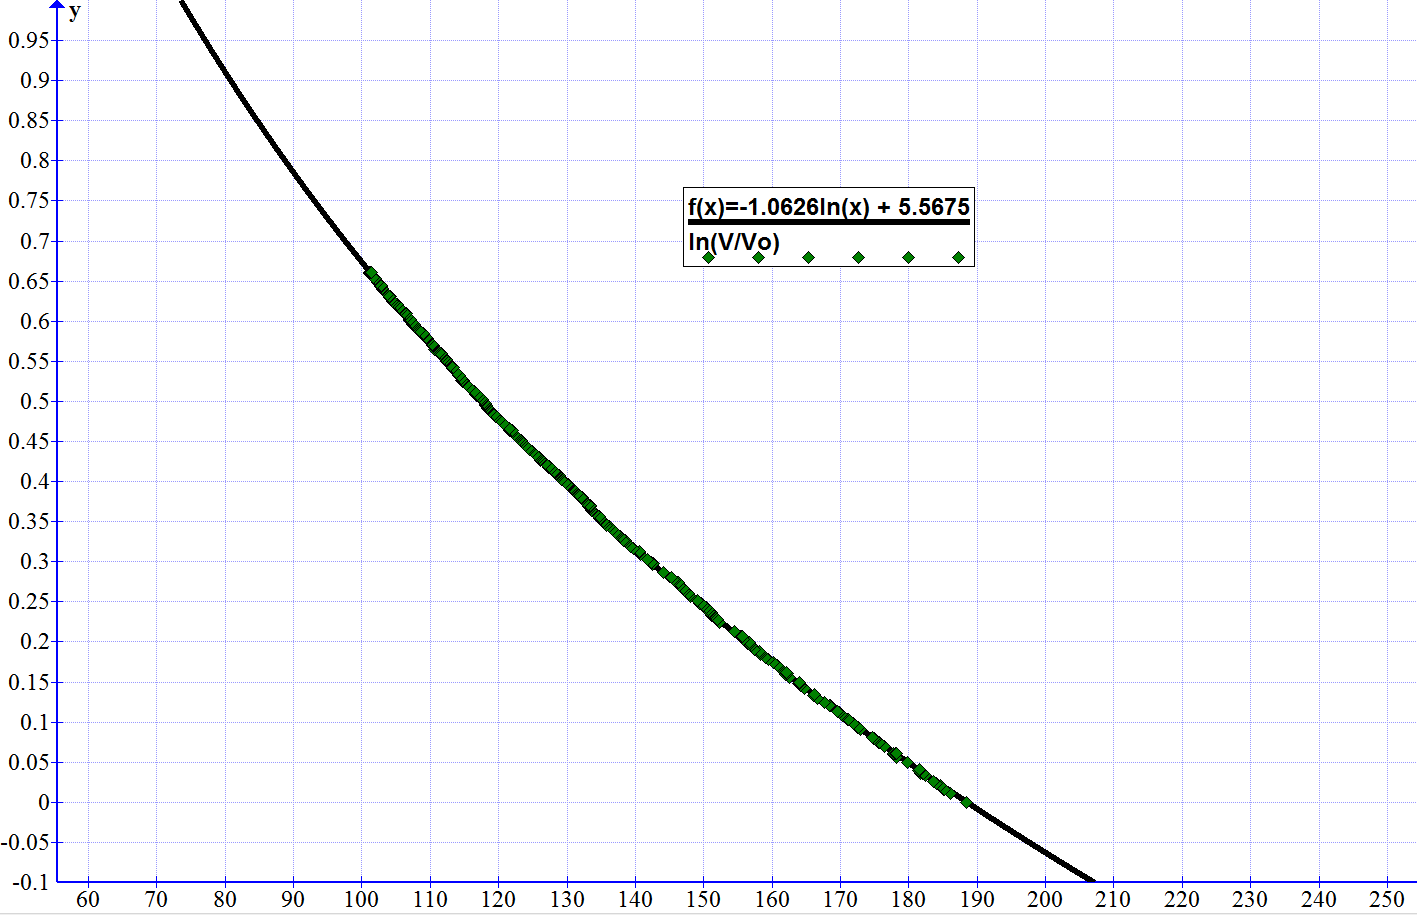
\includegraphics[width=0.75\linewidth]{extra}
	\caption{Relación $ \ln \left(\frac{V}{V_0} \right)$ vs P}
\end{figure}

\begin{figure}[H]
	\centering
	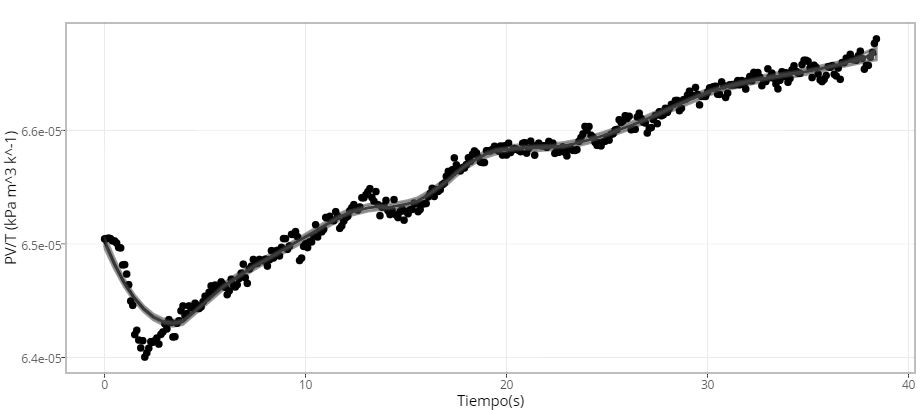
\includegraphics[width=0.75\linewidth]{extra2}
	\caption{Relación $\frac{PV}{T}$ vs Tiempo}
\end{figure}
Si fuera un comportamiento de gas ideal debería ser una recta horizontal ya que por su ecuación de de estado $\frac{PV}{T} = nR$, donde $n$ es el numero de moles y $R$ es la constante de los gases. $n$ no puede cambiar ya que el sistema se encuentra asilado, y $R$ es constante.
\end{document}